\let\negmedspace\undefined
\let\negthickspace\undefined
\documentclass[journal]{IEEEtran}
\usepackage[a5paper, margin=10mm, onecolumn]{geometry}
\usepackage{lmodern} % Ensure lmodern is loaded for pdflatex
\usepackage{tfrupee} % Include tfrupee package

\setlength{\headheight}{1cm} % Set the height of the header box
\setlength{\headsep}{0mm}     % Set the distance between the header box and the top of the text

\usepackage{gvv-book}
\usepackage{gvv}
\usepackage{cite}
\usepackage{amsmath,amssymb,amsfonts,amsthm}
\usepackage{algorithmic}
\usepackage{graphicx}
\usepackage{textcomp}
\usepackage{xcolor}
\usepackage{txfonts}
\usepackage{listings}
\usepackage{enumitem}
\usepackage{mathtools}
\usepackage{gensymb}
\usepackage{comment}
\usepackage[breaklinks=true]{hyperref}
\usepackage{tkz-euclide} 
\usepackage{listings}
\def\inputGnumericTable{}                                 
\usepackage[latin1]{inputenc}                                
\usepackage{color}                                            
\usepackage{array}                                            
\usepackage{longtable}                                       
\usepackage{calc}                                             
\usepackage{multirow}                                         
\usepackage{hhline}                                           
\usepackage{ifthen}                                           
\usepackage{lscape}

\begin{document}

\bibliographystyle{IEEEtran}
\vspace{3cm}

\title{9.1.3}
\author{EE24BTECH11002 - Agamjot Singh}
% \maketitle
% \newpage
% \bigskip
{\let\newpage\relax\maketitle}

\renewcommand{\thefigure}{\theenumi}
\renewcommand{\thetable}{\theenumi}
\setlength{\intextsep}{10pt} % Space between text and floats

\textbf{Question:}
\newline
Solve the differential equation:
\begin{align}
    \brak{\frac{dy}{dx}}^4 + 3y{\frac{d^2 y}{d x^2}} = 0
\end{align}

\textbf{Solution:}

Theoritical solution:
TODO
\newline
Computational Solution: Euler's method
\newline
By the first principle of derivative,
\begin{align}
    y^{\prime}\brak{x} &= \lim_{h\to0} \frac{y\brak{x + h} - y\brak{x}}{h}\\
    y\brak{x + h} &= y\brak{x} + h\brak{y^{\prime}\brak{x}}, h\to0
\end{align}

For a $m^{\text{th}}$ order differential equation,
\newline
Let $y_1 = y$, $y_2 = y^{\prime}$, $y_3 = y^{\prime\prime} \dots$, $y_m = y^{m - 1}$, then we obtain the system
\begin{align}
    \myvec{y_1^{\prime}\\y_2^{\prime}\\\vdots\\y_{m - 1}^{\prime}\\y_m^{\prime}} = \myvec{y_2\\y_3\\\vdots\\y_m\\f\brak{x, y_1, y_2,\dots,y_m}}
\end{align}
Here, $f$ is described by the given differential equation. The initial conditions $y_1\brak{x_0} = K_1$, $y_2\brak{x_0} = K_2$, $\dots$, $y_m\brak{x_0} = K_m$.

Using Euler's method \brak{\text{first principle of derivative}},
\begin{align}
    \myvec{y_1\brak{x + h}\\y_2\brak{x + h}\\\vdots\\y_m\brak{x + h}} = \myvec{y_1\brak{x} + hy_2\brak{x}\\y_2\brak{x} + hy_3\brak{x}\\\vdots\\y_m\brak{x} + hf\brak{x, y_1, y_2 \dots y_m}}
\end{align}

The given differential equation can be represented as,
\begin{align}
    \brak{y^{\prime}}^4 + 3yy^{\prime\prime} = 0
\end{align}

\begin{figure}[h!]
   \centering
   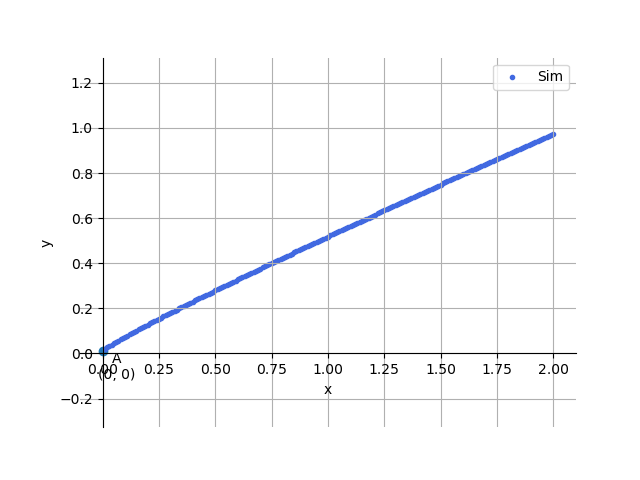
\includegraphics[width=0.7\linewidth]{figs/graph.png}
   \caption{Quadrilateral ABCD formed with given equations}
   \label{label}
\end{figure}

\end{document}
